\documentclass{article}

\usepackage[a4paper, total={6in, 10in}]{geometry}
\usepackage[utf8]{vietnam}
\usepackage{cite}
\usepackage{float}
\usepackage{graphicx}
\usepackage{lmodern}
\usepackage{minted}
\usepackage{hyperref}

\begin{document}
\title{
	\LARGE{
		\textbf{
			Xây dựng mô hình Machine Learning \\ dự báo cháy rừng ở các tỉnh Tây Nguyên \\ dựa vào dữ liệu lịch sử thời tiết.
		}
	}
}

\author{
	Nguyễn Đại Kỳ\\
	19521731\\
	\and
	Văn Viết Hiếu Anh\\
	19521225
	\and
	Lê Văn Phước\\
	19522054
}

\date{\today} % Date for the report
\maketitle % Insert the title, author and date
\begin{center}
	\begin{tabular}{l l}
		Môn học:              & CS114 - Máy học       \\
		Giảng viên hướng dẫn: & Lê Đình Duy           \\
		                      & Phạm Nguyễn Trường An \\
	\end{tabular}
\end{center}

\tableofcontents

\pagebreak

%----------------------------------------------------------------------------------------
%	SECTION 1
%----------------------------------------------------------------------------------------

\section{Tổng quan}
\qquad Bài viết là về quá trình thực nghiệm nghiên cứu các model Machine Learning với mục đích chọn ra mô hình tối ưu để dự đoán mức độ cháy rừng dựa vào dữ liệu thời tiết trong lịch sử của từng địa phương. Với mục đích hổ trợ trong việc dự đoán để phục vụ trong công tác phòng chống cháy rừng ở nước ta. Vì bài viết là ghi chép của quá trình thực nghiệm nên sẽ có nhiều phương pháp được đưa ra sử dụng.

\subsection{Mô tả bài toán}
\qquad Ở nước ta có 3 thảm họa lớn nhất, gây thiệt hại lớn hàng năm về cả người và của. Cùng với lũ lụt và hạn hán, cháy rừng là một thảm họa gây thiệt hại không chỉ về kinh tế mà còn cả con người và hệ sinh thái. Theo thống kê của Cục Kiểm lâm từ năm 1992 đến 2006, trung bình mỗi năm xảy ra 1254 vụ cháy rừng gây thiệt hại khoảng 6646 ha rừng, trong đó có 2854 ha là rừng tự nhiên và 3791 ha là rừng trồng. Bên cạnh việc nâng cao năng lực phòng cháy chữa cháy rừng (PCCCR) cho lực lượng kiểm lâm như đầu tư trang thiết bị, cơ sở vật chất, xây dựng cơ chế điều hành phối hợp và tuyên truyền nâng cao nhận thức trách nhiệm của chủ rừng và người dân, công tác cảnh báo nguy cơ cháy rừng cũng như tổ chức phát hiện sớm và thông báo kịp thời điểm cháy rừng là rất cần thiết.

Từ đầu năm 2007, Cục Kiểm lâm (Bộ Nông nghiệp và Phát triển Nông thôn) đã lắp đặt và vận hành trạm thu ảnh viễn thám MODIS tại Hà Nội với mục đích chính là phát hiện sớm các điểm cháy rừng (hotspots) trên toàn lãnh thổ Việt Nam. Hệ thống trạm thu của TeraScan đã tự động thu nhận, xử lý và sao lưu dữ liệu ảnh MODIS hàng ngày từ 2 vệ tinh TERRA và AQUA với mô-đun Vulcan tự động xử lý và tạo ra dữ liệu các điểm cháy sử dụng thuật toán ATBD-MOD14\cite{website:atbd-mod14}.

Hệ thống này cung cấp dữ liệu về điểm cháy ghi nhận được từ vệ tinh và lưu lại thời gian và tọa độ cháy. Từ khi bắt đầu lắp đặt đến nay hệ thống dữ liệu cháy của cục kiểm lâm được ghi lại được gần 1 triệu điểm cháy. Nhờ lượng dữ liệu này việc xây dựng một hệ thống tự động phân tích mức độ cháy rừng dựa vào các đặc trưng cơ bản của dữ liệu khí tượng thủy văn là hoàn toàn có cơ sở và khả quan.

Input của bài toán là dữ liệu lịch sử thời tiết trong vòng 1 tháng trở lại và từ đó để model đánh giá địa phương đó vào ngày mai có mức độ cháy được đánh giá ở thang nào.

Chưa làm xong đâu, làm phụ đi

\subsection{Mô tả dữ liệu}

Nguồn dữ liệu của nhóm đến từ các website gồm 3 website chính:

\begin{itemize}
	\item firewatchvn.kiemlam.org.vn: là Hệ thống theo dõi cháy rừng trực tuyến thuộc Cục Kiểm Lâm - Tổng cục Lâm Nghiệp
	\item weather.com: là website của The Weather Channel (TWC) - IBM\cite{website:wiki_twc}
	\item worldweatheronline.com
\end{itemize}

Trong 3 nguồn dữ liệu thì chỉ có worldweatheronline.com sử dụng SSR(Server-side render) còn 2 nguồn còn lại đều sử dụng Ajax để truyền dữ liệu qua lại giữa server.

\subsubsection{Weather Data}
\qquad\emph{Việc tìm các nguồn dữ liệu khác về thời tiết ngoài 2 nguồn trên đã được thực hiện song các nguồn này đều có những điểm thiếu rất quan trọng ví dụ như API của website chỉ cung cấp trong 1 năm trở lại hay các website này không cung cấp đủ nhiều địa phương mà chỉ cung cấp dữ liệu ở những thành phố cụ thể.}

Có thể nói việc lấy dữ liệu thời tiết là công đoạn gây ra nhiều khó khăn nhất. Đa phần dữ liệu lịch sử thời tiết là rất lớn và các công ty hay tập đoàn công nghệ đều dùng để bán chứ không public trên website của họ. Ngay cả trên giao diện chính của weather.com của IBM cũng chỉ hiển thị dữ liệu thời tiết trong 2 năm trở lại (tức là 2021 và 2020).

Tuy nhiên vì sử dụng Ajax nên sau khi phân tích và ghi lại các request mà website gửi đi cũng như các response nhận về, việc có thể tìm được các cổng API và phương thức giao tiếp với server, từ đó dùng vào việc khai thác dữ liệu tự động trong nhiều năm trước nữa là hoàn toàn có hy vọng.

Về việc tìm nguồn dữ liệu tương tự đã được khai thác trước, nhóm đã từng thử tìm kiếm nhưng để đạt được yêu cầu chi tiết đến từng địa phương với thời gian kéo dài thì không tìm được dữ liệu nào đạt yêu cầu. Ngay cả khi join vào Slack của \href{https://callforcode.org/}{Call For Code} năm nay để xin hỗ trợ vì đề tài này có liên quan đến cuộc thi thì phía ban tổ chức cuộc thi cũng trả lời rằng dữ liệu này không cung cấp cho thí sinh. Ngoài ra nhóm cũng đã thử gửi mail cho Trung tâm Dự báo khí tượng thuỷ văn quốc gia nhưng cũng không nhận được phản hồi. Hiển nhiên, việc tự đi thu thập dữ liệu là tất yếu.

\subsubsection{Fire Data}
\qquad firewatchvn.kiemlam.org.vn là website tạo ra ý tưởng cho nhóm. Website này cung cấp giao diện tra cứu dữ liệu về các điểm cháy vào từng thời gian cụ thể. Tuy nhiên điểm yếu của website này là xây dựng quá nhiều tính năng và sử dụng Ajax nên dùng những công cụ như Beautiful Soup thì không thể thu thập còn nếu dùng những công cụ như Selenium hay Puppeteer thì tốc độ quá chậm (dữ liệu này kéo dài từ 1/1/2008 đến 5/12/2020 nếu tra cứu từng ngày trên 700 quận, huyện, thành phố thuộc tỉnh,... thì sẽ mất rất nhiều thời gian). Điều này bắt buộc nhóm phải phân tích API mà website đã lấy dữ liệu điểm cháy để tăng tốc độ lấy dữ liệu. Bởi vì những thông tin như bản đồ của địa điểm lấy dữ liệu là không cần thiết, ta hoàn toàn có thể lấy bản đồ địa hình của cả trái đất chỉ cần dùng tọa độ. Việc lấy những thông tin nặng như bản đồ cần thời gian tải rất lâu nên việc tìm ra API mà website sử dụng cũng là cần thiết.


%----------------------------------------------------------------------------------------
%	SECTION 2
%----------------------------------------------------------------------------------------

\section{Các nghiên cứu trước}
% Chương này trình bày các kết quả nghiên cứu đã có của tiền nhân liên quan đến bài toán mà nhóm chọn. Những nghiên cứu trước làm trên các bộ dữ liệu nào, dùng phương pháp nào và performance đạt được bao nhiêu
% Nếu có khả năng thì phân tích thêm kết quả của họ như vậy là tốt chưa, có còn chỗ gì để cải thiện không. Nếu không nhận xét dược thì thôi.
\subsection{Predicting Australia wildfires with weather data a Call For Code spot challenge of IBM}
Mục đích của cuộc thi này là dự đoán kích thước của khu vực cháy tính bằng km2 theo khu vực ở Úc cho mỗi ngày trong tháng 2 năm 2021 bằng cách sử dụng dữ liệu có sẳn cho đến ngày 29 tháng 1.
Bài toán chuỗi thời gian dựa trên dữ liệu hàng ngày do Pairs Geoscope cung cấp.
Dữ liệu được cung cấp bao gồm:
\begin{itemize}
	\item Những trận cháy rừng trong lịch sử
	\item Thời tiết lịch sử
	\item Các dự báo thời tiết lịch sử
	\item Chỉ số thảm thực vật lịch sử
	\item Các loại đất của các địa điểm xảy ra cháy rừng.
\end{itemize}
Trong đó dữ liệu thời tiết lịch sử bao gồm các trường như \textbf{vùng}, \textbf{thời gian}, \textbf{lượng mưa (mm/ngày)}, \textbf{Độ ẩm tương đối (\%)}, \textbf{Hàm lượng nước trong đất ($m^3$/$m^3$)}, \textbf{bức xạ mặt trời (MJ/ngày)}, \textbf{nhiệt độ (C)}, \textbf{tốc độ gió (m/s)}. Đây là dữ liệu chính áp dụng vào bài toán của nhóm. Tuy nhiên vì khó khăn trong việc tìm kiếm dữ liệu nên nhóm chỉ đáp 4/6 tiêu chí mà các chuyên gia đã đưa ra đó là lượng mưa, độ ẩm, nhiệt độ, tốc độ gió.

Từ những nghiên cứu các chuyên gia đưa ra các biến ảnh hưởng đến cháy rừng như:
\begin{itemize}
	\item Lãnh thổ:
	      \begin{itemize}
		      \item Khu vực: Số lượng và cường độ đám cháy khác nhau ở các khu vực khác nhau. Các sự kiện ở các khu vực lân cận có thê ảnh hưởng đến cháy rừng trong một lãnh thổ nhất định. Thành phần tự phục hồi( sự diện diện của cháy rừng trong những ngày trước đó).
		      \item Tính theo mùa: Cháy rừng đặc biệt dữ dội trong “Mùa cháy rừng” kéo dài từ tháng 10 đến tháng 12. Quan sát này sẽ ảnh hưởng đến cách thức phân chia tập dữ liệu huấn luận và kiểm tra.
	      \end{itemize}
	\item Điều kiện đất và khí quyển:
	      \begin{itemize}
		      \item Thời tiết và đất đai: Thời tiết và Hạn hán có liên quan chặt chẽ đến hỏa hoạn. So sánh giữa lịch sử và dự báo thời tiết trong lịch sử.
		      \item Thảm thực vật: Có mối tương quan thuận giữa sự thay đổi chỉ số thảm thực vật và cường độ cháy.
		      \item Sử dụng đất: Việc sử dụng đất có thể liên quan đến việc dự đoán sự kéo dài của cháy rừng. Tuy nhiên, dữ liệu này chỉ có sẳn dưới dạng một hàng – cho mọi khu vực, do đó nó không được đưa vào mô hình.
	      \end{itemize}
\end{itemize}
Theo báo các tổng kết cuộc thi thì mô hình được sử dụng là Convolutional Neural Network (Windowing Dataset, Conv1D Layers,…) cho ra kết quả RMSE: 19.96, MAE: 6.94, TOT: 9.54
Qua nghiên cứu của cuộc thi này nhóm rút ra được các biến ảnh hưởng đến cháy rừng, cách khai thác lấy dữ liệu từ thực tế, mô hình đào tạo phù hợp với bài toán.
\subsection{AI and Climate data for predicting fire frequency in California}
Mục đích của nghiên cứu này là dự đoán tần suất xảy ra cháy rừng có thể giúp lập kế hoạch khẩn cấp và chủ động quản lý rủ ro thiên tai.
Dữ liệu về đám cháy được thu từ Kaggle(\url{https://www.kaggle.com/rtatman/188-million-us-wildfires}), bao gồm khoảng 1,9 triệu vụ cháy rừng ở Mỹ được tham chiếu trong giai đoạn 1992-2015. Ngoài ra, dữ liệu khí hậu từ Copernicus ERA5 được tải xuống và sử dụng cho bài toán này.

Bài nghiên cứu này cũng đưa ra kết luận về việc cháy rừng thường xảy ra hàng tháng hoặc theo mùa. Ở đây, các chuyên gia đưa ra các trường dữ liệu thời tiết được lấy là \textbf{total\_precipitation (tổng lượng mưa)}, \textbf{2m\_temperature (nhiệt độ)}, \textbf{2m\_dewpoint\_temperature (nhiệt độ điểm sương)}, \textbf{10m\_wind\_speed (tốc độ gió)}, \textbf{volumetric\_soil\_water (lượng nước trong đất)}, \textbf{potential\_evaporation (khả năng bốc hơi)}.

Qua nghiên cứu, bài báo đã tính toán hệ số tương quan giữa tuần suất các đám cháy và điều kiện khi hậu trung bình. Phân tích chỉ ra mối tương quan cao đáng kể giữa nhiệt độ mùa hè và PET với số lượng các sự kiện cháy ở CA.

Mô hình dữ đoán trong nghiên cứu này khá đơn giản và nó chỉ sử dụng 6 biến khi hậu được tính trung bình trên toàn California để dự đoán tần suất cá đám cháy trong tiểu bang. Sử dụng tensorflow và scikit-learning để phát triển mạng nơ-ron nhân tạo dựa trên hồi quy.

Từ đánh giá mô hình của bài nghiên cứu cho ra sai số tuyệt đối trung bình tương đối hàng năm (RMAE) khoảng 10\%.

Qua nghiên cứu trên, nhóm cũng rút ra được các biến dữ liệu cần thiết và tác động lớn đến cháy rừng, các phương pháp xử lý số liệu và mô hình được đề xuất sử dụng cho loại bài toán này là ANN.
%----------------------------------------------------------------------------------------
%	SECTION 3
%----------------------------------------------------------------------------------------
\section{Xây dựng bộ dữ liệu}
% Chương này mô tả quá trình thu thập dữ liệu. Nếu dữ liệu crawling tự động thì mô tả cách viết crawler, các khó khăn gặp phải và các số liệu liên quan. Nếu dữ liệu thu thập thủ công thì mô tả các tiêu chí đặt ra để thống nhất trong nhóm khi thu thập. Làm sao để đảm bảo bộ dữ liệu thu thập thủ công có thể khớp gần giống với ngữ cảnh ứng dụng của bài toán.

% Sau đó mô tả các thông số chi tiết của bộ dữ liệu, kèm theo ví dụ minh họa rõ ràng. Bài toán đặt ra các trường hợp dữ liệu nào là khó xử lý, có bao nhiêu mẫu dữ liệu thuộc trường hợp đó, chụp vài mẫu dữ liệu khó đó vào báo cáo để minh họa.

\emph{Lưu ý ở phần này Tỉnh là thuật ngữ để chỉ chung đơn vị hành chính cấp 1 trực thuộc quốc gia, thay cho "tỉnh thành" hoặc chính xác hơn là "đơn vị hành chính cấp tỉnh". Tương tự với "Huyện" là đơn vị hành chính bậc hai, và xã là cấp ba.}


\subsection{Quá trình thu thập dữ liệu}

Tất cả dữ liệu của nhóm đều bắt đầu bằng 1 quy trình chung để kiểm tra xem nguồn dữ liệu có đáp ứng các yêu cầu hay không.

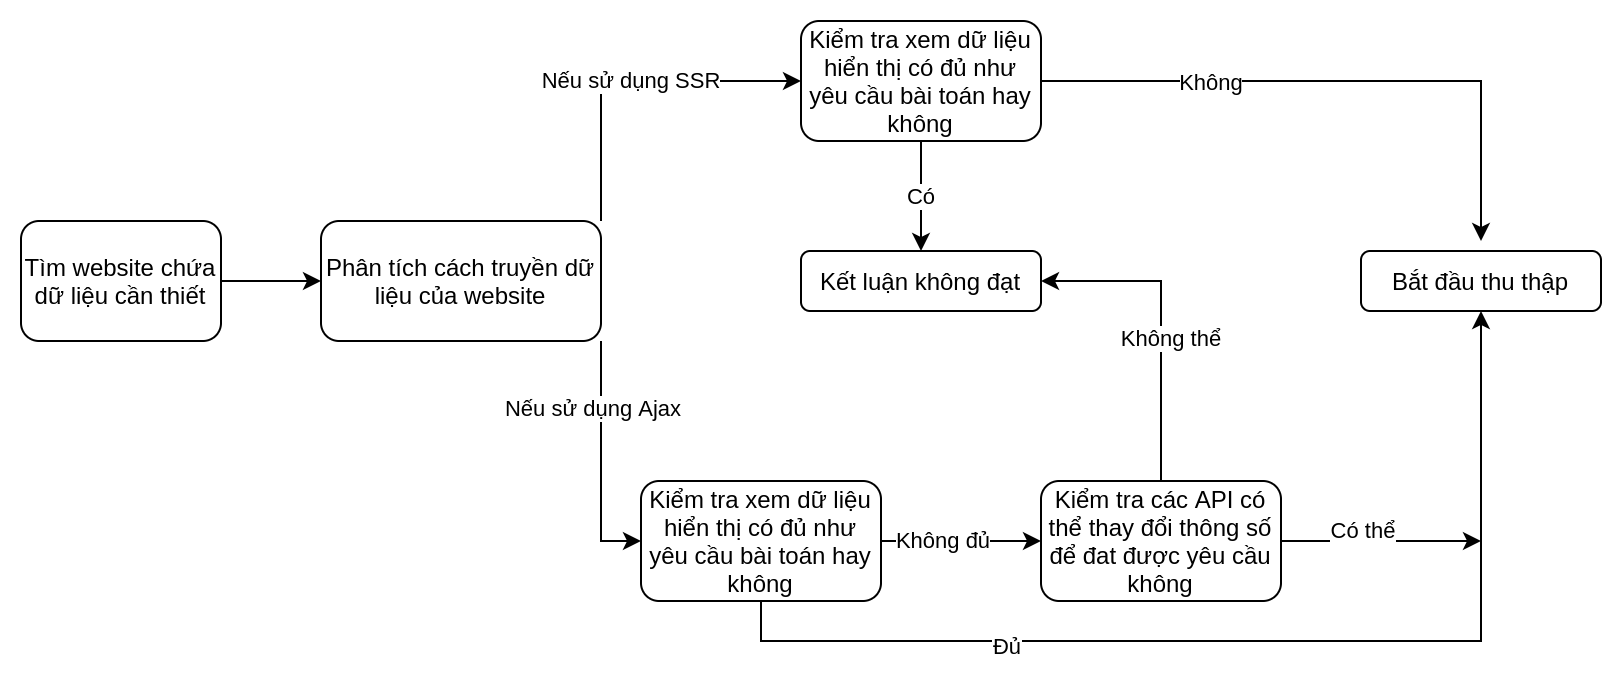
\includegraphics[width=6in]{images/process.png}

\subsubsection{weather.com}
\qquad Để tìm ra API phục vụ cho việc crawl ta vào trang Monthly của một địa phương cụ thể sau đó navigate đến các trang chứa dữ liệu của các tháng trước (việc này giúp cho website sử dụng các API yêu cầu dữ liệu thời tiết quá khứ). Kiểm tra các response trong filter XHR ta có thể tìm ra những response tốt nhất chứa dữ liệu cần thiết.

\begin{figure}[H]
	\centering
	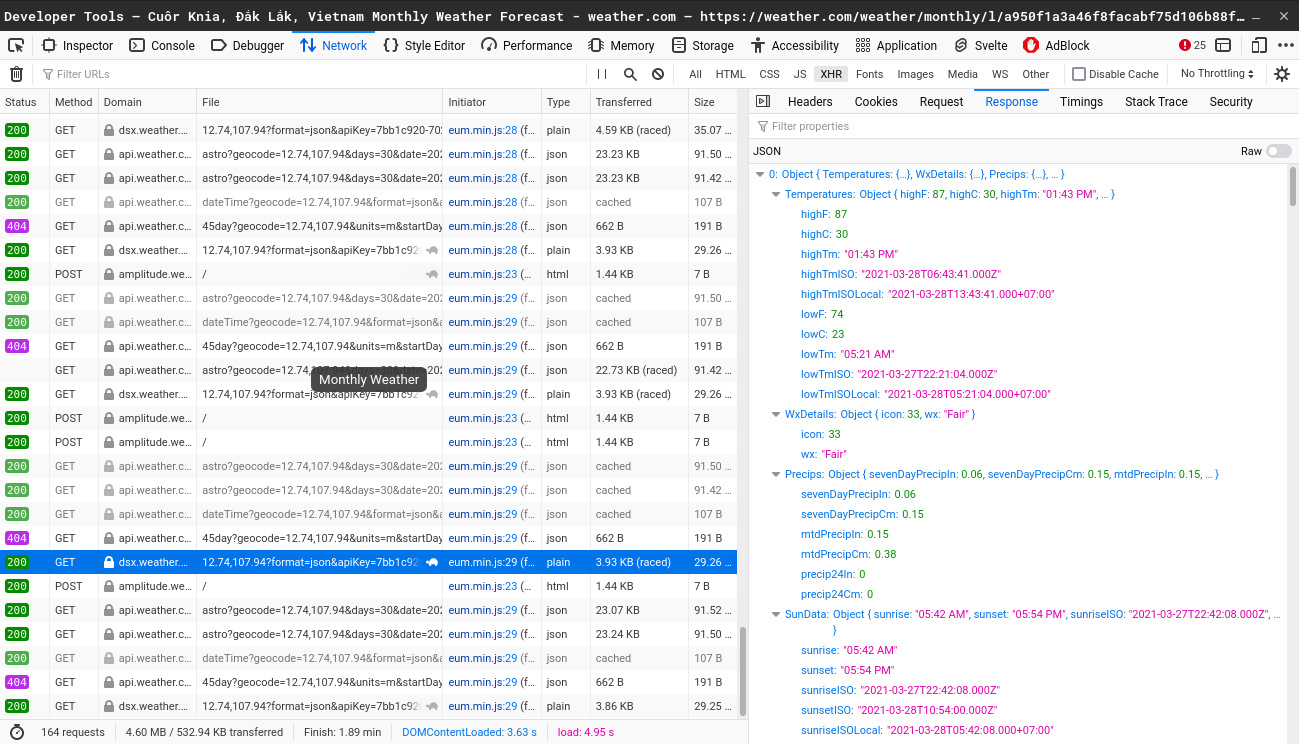
\includegraphics[width=6in]{images/inspect.png}
	\caption{Thông tin của response chứa những thông tin cần thiết}
\end{figure}

Tiếp theo đó khi đã xác nhận API này đủ điều kiện ra kiểm tra ý nghĩa của các thông số trong request, thử thay đổi thông số để kiểm tra dữ liệu kéo dài được đến bao lâu.


\begin{figure}[H]
	\centering
	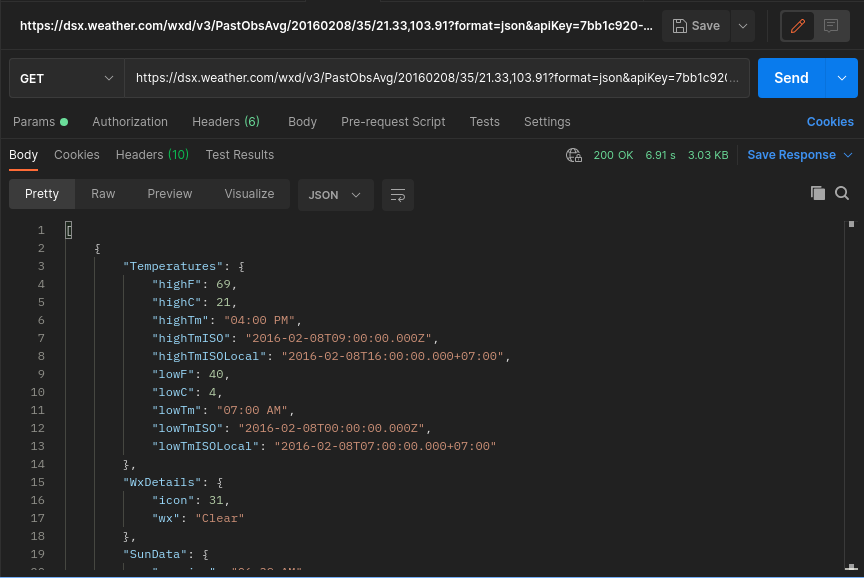
\includegraphics[width=6in]{images/checkpast.png}
	\caption{Thử nghiệm với các tham số khác}
\end{figure}

Vì dữ liệu chấp nhận đến 2014 nên sẽ tiến hành crawl dữ liệu. Nhóm sử dụng Scrappy để crawl vì công cụ này hỗ trợ async cho phép gửi nhiều request cùng lúc cùng với đó là có pipeline để lưu dữ liệu nên giảm rất nhiều quá trình cài đặt.

% Continue here
Đầu tiên ta tạo tải dữ liệu danh sách chứa tất cả các xã cần crawl dữ liệu, làm tròn các tọa độ đến 2 chữ số thập phân(theo yêu cầu của API, xử lý bằng numpy trước sẽ nhanh hơn việc xử lý trong vòng lặp).

\begin{minted}[tabsize=4,breaklines]{python}
class IBMWeatherScapper(Spider):
    name = 'ibm-weather'

    df_ward_taynguyen_fire = pandas.read_csv(
        'https://raw.githubusercontent.com/.../taynguyen_wards_longlat.csv')
    df_ward_taynguyen_fire['long'] = numpy.round(
        df_ward_taynguyen_fire['long'], 2)
    df_ward_taynguyen_fire['lat'] = numpy.round(
        df_ward_taynguyen_fire['lat'], 2)
\end{minted}

Trong hàm start\_requests của Spider với mỗi xã ta tạo 1 request vào ngày 1/1/2014 với tọa độ của xã đó, cùng với đó là lưu kèm 1 meta để nhận diện xã đó trong parse function.

\begin{minted}[tabsize=4,breaklines]{python}
	def start_requests(self):
	requests = []
	for i, ward in self.df_ward_taynguyen_fire.iterrows():
		requests.append(request.Request(
			url=f"https://dsx.weather.com/wxd/v3/PastObsAvg/20140101/35/\
			{ward['lat']:.2f},{ward['long']:.2f}\
			?format=json\
			&apiKey=7bb1c920-7027-4289-9c96-ae5e263980bc&\
			fbclid=IwAR1IgpD8qPU6ZaHqDnZT1tMl95Y4G8gfGvIYmpM3CGGIqyjwQeaAmbZZ8SE",
			meta={
				'ward_code': ward['ward_code'],
				'long':ward['long'],
				'lat':ward['lat']
			},
			callback=self.parse
		))
	return requests
\end{minted}

Vì đây là API nên dữ liệu được thể hiện dưới dạng json rất rõ ràng.

\begin{minted}[tabsize=4,breaklines]{javascript}
	{
        "Temperatures": {
            "highF": 72,
            "highC": 22,
            "highTm": "01:00 PM",
            "highTmISO": "2014-01-01T06:00:00.000Z",
            "highTmISOLocal": "2014-01-01T13:00:00.000+07:00",
            "lowF": 68,
            "lowC": 20,
            "lowTm": "01:00 AM",
            "lowTmISO": "2013-12-31T18:00:00.000Z",
            "lowTmISOLocal": "2014-01-01T01:00:00.000+07:00"
        },
        "WxDetails": { "icon": 27, "wx": "Mostly Cloudy" },
        "SunData": {
            "sunrise": "06:05 AM",
            "sunset": "05:26 PM",
            "sunriseISO": "2013-12-31T23:05:00.000Z",
            "sunsetISO": "2014-01-01T10:26:00.000Z",
            "sunriseISOLocal": "2014-01-01T06:05:00.000+07:00",
            "sunsetISOLocal": "2014-01-01T17:26:00.000+07:00"
        },
        "Moon": {
            "moonriseLocal": "2014-01-01T05:34:00.000+07:00",
            "moonsetLocal": "2014-01-01T17:25:00.000+07:00",
            "moonriseISO": "2013-12-31T22:34:00.000Z",
            "moonsetlISO": "2014-01-01T10:25:00.000Z"
        }
    }
\end{minted}

Việc còn lại là lấy ra và lưu lại dưới file csv. Sau đó lấy ngày cuối cùng trong dữ liệu trả về xem có bằng ngày hôm nay không, nếu không thì tiếp tục tải dữ liệu còn nếu có thì dừng lại.

\begin{minted}[tabsize=4]{python}
	 def parse(self, response, **kwargs):
        json = response.json()
        ward_code = response.meta['ward_code']
        long = response.meta['long']
        lat = response.meta['lat']
        for d in json:
            yield {
                'ward':ward_code,
                'date':d.get('Temperatures', {}).get('highTmISOLocal','')[:10],
                'highC': d.get('Temperatures', {}).get('highC',''),
                'lowC': d.get('Temperatures', {}).get('lowC',''),
                'sun_rise': d.get('SunData', {}).get('sunrise',''),
                'sun_set': d.get('SunData',{}).get('sunset',''),
                'sevenDayPrecipCm':d.get('Precips',{}).get('sevenDayPrecipCm',''),
                'mtdPrecipCm':d.get('Precips',{}).get('mtdPrecipCm',''),
                'precip24Cm':d.get('Precips',{}).get('precip24Cm',''),
            }

		last = json[-1]
        recentDate = datetime.strptime(last['Temperatures']['highTmISO'][:10], '%Y-%M-%d')
        next = recentDate + timedelta(days=1)
		
		if recentDate.date() == datetime.today():
        	return
        else:
            yield response.follow(
                url=f"https://dsx.weather.com/wxd/v3/PastObsAvg/ \
				{next.strftime('%Y%M%d')}/35/{lat:.2f},{long:.2f}\
				?format=json\
				&apiKey=7bb1c920-7027-4289-9c96-ae5e263980bc\
				&fbclid=IwAR1IgpD8qPU6ZaHqDnZT1tMl95Y4G8gfGvIYmpM3CGGIqyjwQeaAmbZZ8SE",
                meta={
                        'ward_code': ward_code,
                        'long':long, 'lat':lat
                    },
                    callback=self.parse
            )
\end{minted}

Dữ liệu từ website này cung cấp có độ chính xác đến từng tọa độ, có nghĩa là chỉ cần cung cấp tọa độ (làm tròn đến 2 chữ số thập phân) thì server sẽ trả về thời tiết tại điểm đó tùy vào thời gian mà ta muốn. Tuy nhiên điểm yếu của dữ liệu này là chỉ cung cấp các đặc tính cơ bản nhất của thời tiết tại địa điểm đó gồm: nhiệt độ cao nhất và thấp nhất trong ngày, thời gian mặt trời mọc và lặn, lượng mưa (tích lũy trong 7 ngày, trong 1 tháng hoặc chỉ ngày hôm đó).

Sau khoảng nhiều ngày khai thác và xử lý, nhóm đã lấy được dữ liệu của 5 tỉnh Tây Nguyên vào từng xã từng ngày kéo dài từ 1/1/2014 đến 8/6/2021. Dữ liệu gồm các trường cơ bản sau (lưu ý các trường này đã được đổi tên so với khi crawl dữ liệu để thống nhất các bộ dữ liệu với nhau nhằm dễ dàng cho việc nghiên cứu):

\begin{itemize}
	\item \texttt{ward}: Mã xã. Vì sẽ có những địa điểm trùng tên nên nhóm sử dụng mã để phân biệt các địa phương (mã này cung cấp bởi API của firewatchvn.kiemlam.org.vn\cite{website:firewatch_administrative})
	\item \texttt{date}: là ngày mà record được ghi lại.
	\item \texttt{max/min}: là nhiệt độ cao nhất và thấp nhất được ghi nhận trong ngày(celcius).
	\item \texttt{sunrise/sunset}: là thời gian mặt trời mọc và lặn.
	\item \texttt{7\_rain}: lượng mưa tổng tính từ ngày chủ nhật gần nhất trước đó (cm)
	\item \texttt{m\_rain}: lượng mưa tổng tính từ ngày 1 của tháng đó(cm)
	\item \texttt{24\_rain}: lượng mưa ghi nhận trong ngày(cm)
\end{itemize}

Dưới đây là một đoạn mẫu trong dữ liệu.

\begin{table}[H]
	\begin{tabular}{lllllllll}
		ward    & date       & max & min & sunrise  & sunset   & 7\_rain & m\_rain & 24\_rain \\
		24727.0 & 2016-10-17 & 30  & 25  & 05:36 AM & 05:28 PM & 5.94    & 30.91   & 1.82     \\
		24727.0 & 2016-10-18 & 30  & 25  & 05:36 AM & 05:28 PM & 7.54    & 32.66   & 1.75     \\
		24727.0 & 2016-10-19 & 30  & 25  & 05:36 AM & 05:27 PM & 7.54    & 32.96   & 0.3      \\
		24761.0 & 2019-10-14 & 32  & 24  & 05:36 AM & 05:30 PM & 0.02    & 0.07    & 0.0      \\
		24761.0 & 2019-10-15 & 32  & 25  & 05:36 AM & 05:30 PM & 0.02    & 0.07    & 0.0      \\
		24761.0 & 2019-10-16 & 32  & 25  & 05:36 AM & 05:29 PM & 0.02    & 0.07    & 0.02     \\
		24761.0 & 2019-10-17 & 32  & 25  & 05:36 AM & 05:29 PM & 0.02    & 0.07    & 0.0      \\
		24761.0 & 2019-10-18 & 32  & 25  & 05:36 AM & 05:28 PM & 0.02    & 0.07    & 0.0      \\
		24761.0 & 2019-10-19 & 32  & 26  & 05:36 AM & 05:28 PM & 0.02    & 0.07    & 0.0      \\
		24761.0 & 2019-10-20 & 32  & 26  & 05:36 AM & 05:27 PM & 0.02    & 0.1     & 0.0      \\
		24761.0 & 2019-10-21 & 33  & 25  & 05:36 AM & 05:27 PM & 0.02    & 0.1     & 0.0      \\
		24761.0 & 2019-10-22 & 32  & 25  & 05:37 AM & 05:26 PM & 0.02    & 0.1     & 0.0      \\
		24761.0 & 2019-10-23 & 33  & 25  & 05:37 AM & 05:26 PM & 0.0     & 0.1     & 0.0      \\
		24761.0 & 2019-10-24 & 33  & 25  & 05:37 AM & 05:25 PM & 0.0     & 0.1     & 0.0
	\end{tabular}
\end{table}

Dưới đây là các thông số của bộ dữ liệu

\begin{table}[H]
	\begin{tabular}{lllllll}
		      & ward    & max      & min      & 7\_rain   & m\_rain    & 24\_rain  \\
		count & 1130904 & 1130904  & 1130904  & 679514    & 679514     & 679514    \\
		mean  &         & 30.60013 & 24.66924 & 33.813765 & 82.088195  & 4.797731  \\
		std   &         & 2.836824 & 2.207649 & 71.482188 & 153.732438 & 16.574482 \\
		min   &         & 18       & 14       & 0         & 0          & 0         \\
		25\%  &         & 29       & 23       & 0.5       & 2.2        & 0         \\
		50\%  &         & 31       & 25       & 8.1       & 21.3       & 0         \\
		75\%  &         & 32       & 26       & 34.7      & 88.6       & 2.7       \\
		max   &         & 46       & 36       & 903.7     & 1300.7     & 419.1
	\end{tabular}
\end{table}


\begin{figure}[H]
	\centering
	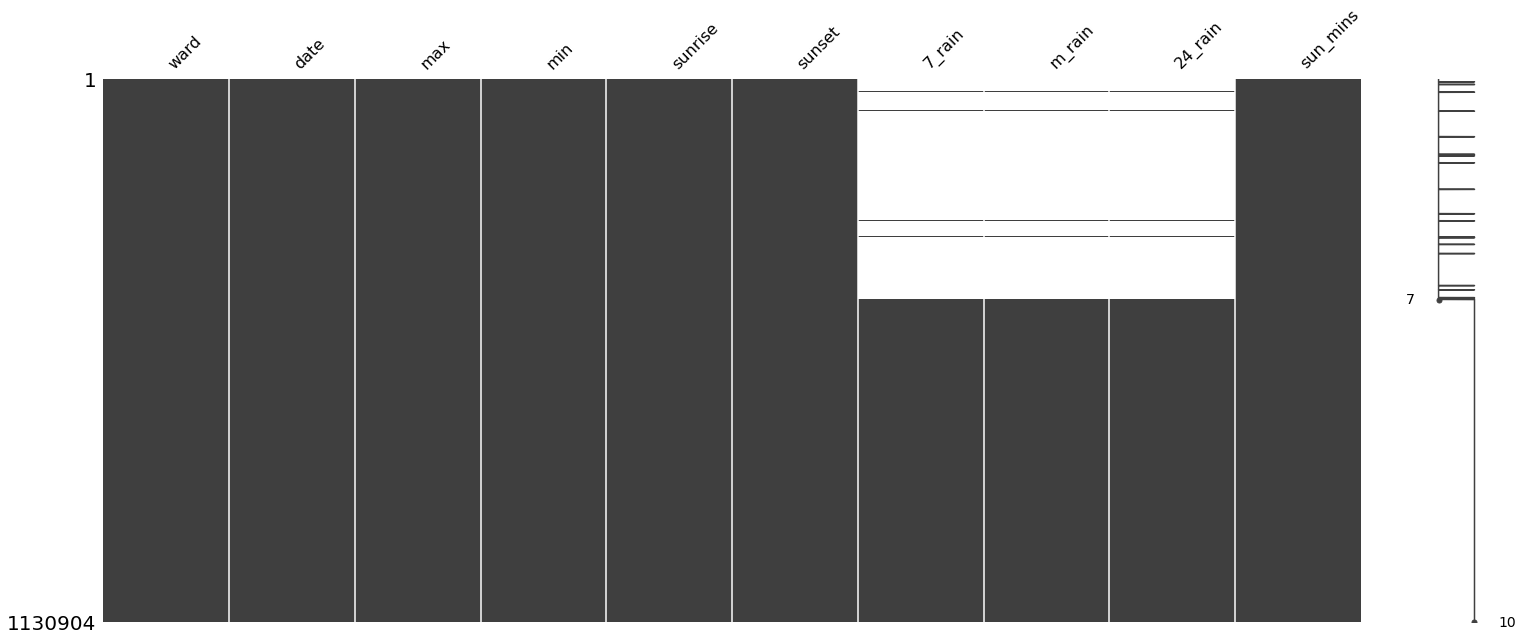
\includegraphics[width=6in]{images/missing.png}
	\caption{
		Dữ liệu sau khi sắp xếp theo ngày và địa phương(theo thứ tự ngày trước địa phương sau, tăng dần). Phần được tô là phần chứa dữ liệu, phần màu trắng là phần dữ liệu trống}
\end{figure}


\subsubsection{worldweatheronline.com}
Ở trang này dữ liệu thời tiết chỉ hiển thị ở 40 tỉnh thành, các điểm dữ liệu này được đặt title theo trung tâm hành chỉnh của tỉnh thành phố đó.

Danh sách 40 thành phố:
\begin{table}[H]
	\begin{tabular}{llll}
		Bac Lieu    & Ho Chi Minh City & Tam Ky    & Ben Tre   \\
		Hoa Binh    & Tan An           & Bien Hoa  & Hong Gai  \\
		Thai Nguyen & Buon Me Thuot    & Hue       & Thanh Hoa \\
		Ca Mau      & Long Xuyen       & Tra Vinh  & Cam Pha   \\
		My Tho      & Tuy Hoa          & Cam Ranh  & Nam Dinh  \\
		Uong Bi     & Can Tho          & Nha Trang & Viet Tri  \\
		Chau Doc    & Phan Rang        & Vinh      & Da Lat    \\
		Phan Thiet  & Vinh Long        & Ha Noi    & Play Cu   \\
		Vung Tau    & Hai Duong        & Qui Nhon  & Yen Bai   \\
		Hai Phong   & Rach Gia         & Hanoi     & Soc Trang \\
	\end{tabular}
\end{table}

\begin{figure}[H]
	\centering
	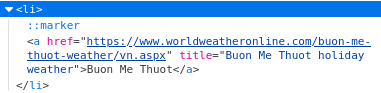
\includegraphics[width=4in]{images/html_structure.png}
	\caption{
		Bố cục danh sách các tỉnh của website, kèm theo đường dẫn trong thẻ a của các tỉnh đó}
\end{figure}

Vì bố cục này đơn giản và hiển thị đầy đủ danh sách trên website nên chỉ cần sử dụng Javascript để lấy danh sách các dường dẫn đến các trang lấy dữ liệu để nhanh hơn trong quá trình xử lý. Trong console của trình duyệt

\begin{minted}[tabsize=4, breaklines]{javascript}
	let a = document.querySelectorAll(".country_part li >a")
	let cities = Array.from(a)
	cities = cities.map(e => {return {title: e.innerHTML, url:e.href}})
	// Dùng stringtify để tạo json string, chuỗi này chính là mảng chứa danh sách các thành phố, ta chỉ cần khai báo như một biến list của dictionary trong python.
	JSON.stringify(cities)
\end{minted}

Dùng phương pháp phân tích tương tự khi phân tích weather.com để kiểm tra thông tin gửi về cho server ta sẽ biết được những thông tin để nhận về thời tiết vào một ngày cụ thể.

\begin{figure}[H]
	\centering
	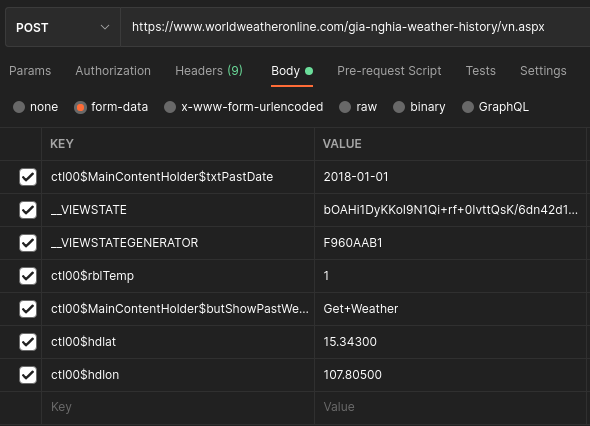
\includegraphics[width=4in]{images/wwo-history-postman.png}
	\caption{
		Những thông số server cần để gửi trả về dữ liệu cần thiết}
\end{figure}

Vì server của website này render hầu như đầy đủ thông tin nên ta chỉ cần lấy thông tin từ mẫu response dưới đây là đạt yêu cầu. Ở đây có thể thấy rằng có một bảng dữ liệu thể hiện sự khác biệt qua từng năm của dữ liệu. Nên ta chỉ cần gửi 365 request là có thể lấy tất cả dữ liệu cần cho mỗi tỉnh.

\begin{figure}[H]
	\centering
	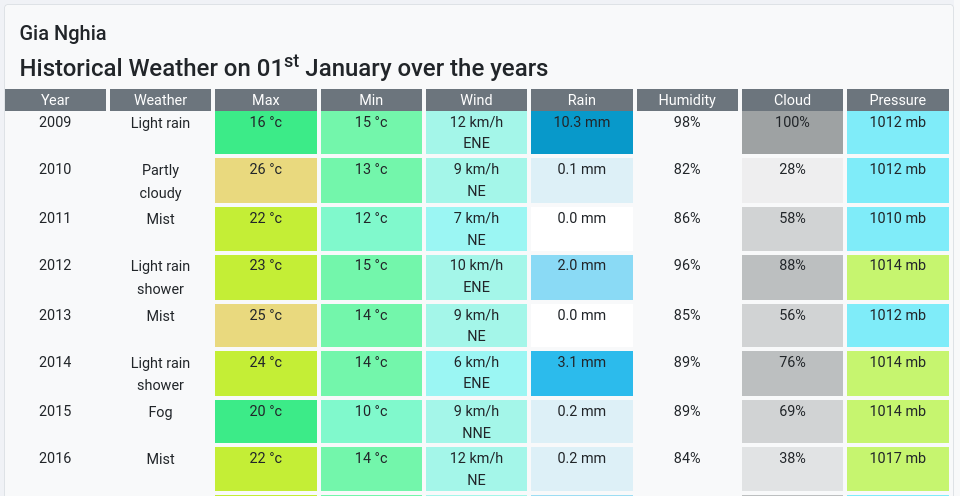
\includegraphics[width=6in]{images/wwo-display-data.png}
	\caption{
		Những dữ liệu response hiển thị}
\end{figure}

Từ những dữ liệu này ta bắt tay vào viết spider.

\begin{minted}[breaklines, tabsize=4]{python}
	# Sử dụng numpy để tạo một mảng chứa tất cả các ngày trong năm 
	BASE = date(2018, 1, 1)
	DATES = numpy.array(
    	[(BASE + timedelta(days=i)).strftime("%Y-%m-%d") for i in range(365)]
	)
\end{minted}

\begin{minted}[breaklines, tabsize=4]{python}
# Các thông số cơ bản của Spider
class WorldWeatherOnlineScraper(Spider):
    name = 'world-weather-online'

    provinces = [
        {
			"url": "https://www.worldweatheronline.com/bac-lieu-weather-history/vn.aspx",
			"title": "Bac Lieu"
		},
		...
		{
			"url": "https://www.worldweatheronline.com/ho-chi-minh-city-weather-history/vn.aspx",
			"title": "Ho Chi Minh City"
		}

    ]

	def start_requests(self):
		# Ở mỗi tỉnh thành ta gửi 365 request cho 365 ngày trong năm
        for province in self.provinces:
            for date in DATES:
                formData = {
					# Các thông số khác như đơn vị nhiệt độ hay tọa độ gửi request đều giống nhau nên sẽ không ghi chú ở đây
                    'ctl00$MainContentHolder$txtPastDate': date,
                }

                yield FormRequest(province['url'],
                                  formdata=formData,
                                  meta={
                    'date': date,
                    'province': province['title']
                }, callback=self.parse
                )

	def parse(self, response):
		# Tách bảng history
        history = response.css('.row.text-center.wwo-tabular')

		# Với mỗi cell trong bảng ta lấy tất cả ra và gom thành một mảng lớn chung
        # 9 element đầu tiên là tên của 9 cột nên ta loại ra
        records = history.css('.col.mr-1::text').getall()[9:]

		# Việc cuối cùng là lặp qua tất cả các dòng để ghi lại dữ liệu
        for i in range(0, len(records), 9):
            yield{
                'province': response.meta['province'],
                'day': response.meta['date'][8:10],
                'month': response.meta['date'][5:7],
                'year': records[i],
                'max': records[i+1],
				# so on ...
                'pressure': records[i+8],
            }
\end{minted}

Sau khoảng 1 tiếng chạy và điều chỉnh lại ta có bảng dữ liệu sau:
\begin{itemize}
	\item Thời gian: 1/1/2009 to 18/06/2021
	\item Địa lý: 40 thành phố, danh sách đã ghi lại ở trên
	\item { Các trường dữ liệu:
	      \begin{itemize}
		      \item \texttt{province}: Tên thành phố \emph{(không dấu)}
		      \item \texttt{date}: ngày
		      \item \texttt{max}: nhiệt độ cao nhất trong ngày \emph{(celcius)}
		      \item \texttt{min}: nhiệt độ thấp nhất trong ngày \emph{(celcius)}
		      \item \texttt{wind}: tốc độ gió \emph{(km/h)}
		      \item \texttt{wind\_d}: hướng gió \href{https://www7.ncdc.noaa.gov/climvis/help_wind.html}{direction}
		      \item \texttt{rain}: lượng mưa \emph{(mm)}
		      \item \texttt{humidi}: độ ẩm \emph{(\%)}
		      \item \texttt{cloud}: mây \emph{(\%)}
		      \item \texttt{pressure}: áp suất(\href{https://en.wikipedia.org/wiki/Bar_(unit)}{Bar})
	      \end{itemize}
	      }
\end{itemize}
Dưới đây là một đoạn trong dữ liệu:
\begin{table}[H]
	\begin{tabular}{llllllllll}
		province & max & min & wind & wind\_d & rain & humidi & cloud & pressure & date       \\
		Bac Lieu & 27  & 22  & 17   & NNE     & 6.9  & 90     & 71    & 1010     & 2009-01-01 \\
		Bac Lieu & 31  & 25  & 20   & ENE     & 0.0  & 64     & 24    & 1010     & 2010-01-01 \\
		Bac Lieu & 29  & 24  & 14   & E       & 0.0  & 75     & 45    & 1008     & 2011-01-01 \\
		Bac Lieu & 30  & 24  & 30   & E       & 0.0  & 79     & 52    & 1012     & 2012-01-01 \\
		Bac Lieu & 31  & 25  & 20   & ENE     & 0.0  & 70     & 24    & 1010     & 2013-01-01
	\end{tabular}
\end{table}

Các thông số cơ bản của dữ liệu (lưu ý rằng gió đã được đổi ra các góc theo radian)

\begin{table}[H]
	\begin{tabular}{lllllllll}
		      & max       & min       & wind      & wind\_d  & rain      & humidi    & cloud     & pressure    \\
		count & 181960    & 181960    & 181960    & 181960   & 181960    & 181960    & 181960    & 181960      \\
		mean  & 29.837277 & 23.277874 & 11.038657 & 2.67885  & 6.56713   & 77.083068 & 41.721268 & 1010.229127 \\
		std   & 4.571345  & 3.945381  & 5.311807  & 1.241257 & 13.602055 & 9.288553  & 23.875067 & 4.635714    \\
		min   & 4         & 2         & 1         & 0        & 0         & 23        & 0         & 988         \\
		25\%  & 28        & 21        & 7         & 1.570796 & 0.1       & 71        & 23        & 1008        \\
		50\%  & 31        & 24        & 10        & 2.356194 & 1.8       & 78        & 38        & 1010        \\
		75\%  & 33        & 26        & 14        & 3.926991 & 7.5       & 83        & 58        & 1012        \\
		max   & 46        & 32        & 54        & 5.890486 & 596.4     & 100       & 100       & 1038
	\end{tabular}
\end{table}

\subsubsection{firewatchvn.kiemlam.org.vn}

Tương tự với 2 trang ở trên, sau khi phân tích dữ liệu nhận về từ các response, ta biết được các cổng API sau:

Domain: \texttt{firewatchvn.kiemlam.org.vn}

\begin{enumerate}
	\item Thông tin cấu trúc hành chính
	      \begin{itemize}
		      \item Route: \texttt{/fwdata/hanhchinh/{province-code}/{district-code}}
		      \item Parameters:
		            \begin{itemize}
			            \item \texttt{province-code}: mã tỉnh, nếu để là 0 thì sẽ trả về danh sách tất cả các tỉnh trên cả nước
			            \item \texttt{district-code}: mã huyện, nếu để là 0 thì sẽ trả về danh sách tất cả các huyện của tỉnh hiện tại, nếu \textbf{ \texttt{province-code} là 0 thì tham số này không có ý nghĩa}
		            \end{itemize}
		      \item Response:
		            \begin{minted}[tabsize=4, breaklines]{javascript}
					// Response from "/fwdata/hanhchinh/0/0"
					[
						{"ma":"89","ten":"An Giang"},
						{"ma":"24","ten":"Bắc Giang"},
						...,
						{"ma":"15","ten":"Yên Bái"}
					]
					\end{minted}
	      \end{itemize}

	\item Thông tin điểm cháy
	      \begin{enumerate}
		      \item Route: {\texttt{/fwdata/search/diaphuong/\{province-code\}/\{district-code\}/\{ward-code\}/}
		            \linebreak
		            \texttt{\{start-date\}/\{end-date\}/1/100}
		            }
		      \item Parameters:
		            \begin{itemize}
			            \item \texttt{province-code}: mã tỉnh, nếu để là 0 thì sẽ trả về thống kê bằng tổng số các vụ cháy trên cả nước ở các tỉnh
			            \item \texttt{district-code}: mã huyện, nếu để là 0 thì sẽ trả về thống kê bằng tổng số các vụ cháy trên cả nước ở các huyện, nếu \texttt{province-code là 0 thì tham số này không có ý nghĩa}
			            \item \texttt{ward-code}: mã xã, nếu để là 0 thì sẽ trả về thống kê bằng tổng số các vụ cháy trên cả nước ở các xã, nếu \textbf{\texttt{province-code} hoặc \texttt{district-code} là 0 thì tham số này không có ý nghĩa}
			            \item \texttt{start-date}: ngày bắt đầu, format dưới dạng \texttt{dd!mm!yyyy}
			            \item \texttt{end-date}: ngày kết thúc, format dưới dạng \texttt{dd!mm!yyyy}
		            \end{itemize}
		      \item Response:
		            \begin{minted}[tabsize=4, breaklines]{javascript}
// Response from "/fwdata/search/diaphuong/49/512/0/01!10!2019/01!10!2019/1/100"
[
    {
        "sdc": 3,
        "x": 108.023503269442,
        "y": 15.5811098358411,
        "xa": "Hiệp Hòa",
        "hp": [
            { 
				"x": 108.02951,
				"y": 15.56155,
				"idhotspot": "20758-_263b067"
			},
            {
				"x": 108.03237,
				"y": 15.553405,
				"idhotspot": "20758-!ab49a26"
			},
            {
				"x": 108.03386,
				"y": 15.58714,
				"idhotspot": "20758-_c73ffe4"
			}
        ]
    },
	...,
    {
        "sdc": 1,
        "x": 108.014536842611,
        "y": 15.537556163829,
        "xa": "Sông Trà",
        "hp": [
			{ 
				"x": 108.05701,
				"y": 15.53117,
				"idhotspot": "20770-_594ec71"
			}
		]
    }
]

					\end{minted}
	      \end{enumerate}
\end{enumerate}

Với API này ta có 2 hướng giải quyết:
\begin{enumerate}
	\item Tạo request cho tất cả các huyện vào mỗi ngày, việc này sẽ giúp quét hết toàn bộ điểm cháy chi tiết đến từng tọa độ theo ngày. Trong bộ dữ liệu có mã của 710 đơn vị hành chính cấp huyện nếu vậy để quét qua từ 1/1/2008 đến 31/12/2020 (khoảng 4749 ngày) ta cần gửi khoảng 3371790 request
	\item Tạo request thống kê trên ngày cho cả nước, gom tất cả các huyện có cháy trong ngày đó, sau đó tra theo mã huyện đã nhận. Phương pháp này có thể giảm nhưng cũng có thể làm tăng số lượng request tùy các các điểm cháy phân bổ.
\end{enumerate}

Sau khi so sánh 2 phương pháp bằng cách request 30 ngày thì phương pháp thứ 2 cho lượng request chỉ bằng 70\% so với phương pháp thứ nhất. Vì vậy nhóm quyết định chọn phương pháp thứ 2.

Dưới đây là kết quả tổng kết từ crawler (đã lược bỏ, chi tiết xem \href{https://github.com/vanviethieuanh/CS114.L21/blob/920ee0722baa05582e67e05f8e5a2a350b18b956/DoAn/Wildfire/wildfire/scrape-log.txt}{tại đây})

\begin{minted}[]{python}
{
    'downloader/request_count': 3127864,
    'downloader/response_count': 3127864,
    'downloader/response_status_count/200': 3127863,
    'downloader/response_status_count/404': 1,
    'elapsed_time_seconds': 68738.104826,
    'finish_reason': 'finished',
    'item_scraped_count': 997218,
}
\end{minted}

Vậy ta đã giảm được 7.23\% lượng request (243926, khoảng 1.489 tiếng thời gian thực thi)

Đặc điểm chung của bộ dữ liệu này là không thiếu sót ở các cell vì nếu đã được ghi lại ở server thì chắc chắn dữ liệu này đầy đủ thông tin.

\begin{itemize}
	\item Thời gian: 1/1/2008 đến 31/12/2020
	\item Địa lý: Cả nước
	\item { Các trường dữ liệu:
	      \begin{itemize}
		      \item \texttt{date}: Ngày ghi nhận dưới dạng \texttt{yyyy-mm-dd}
		      \item \texttt{province}: Tỉnh ghi nhận
		      \item \texttt{district}: Huyện ghi nhận
		      \item \texttt{ward}: Xã ghi nhận
		      \item \texttt{long}: Kinh độ
		      \item \texttt{lat}: Vĩ độ
	      \end{itemize}
	      }
\end{itemize}

Một đoạn mẫu trong dữ liệu
\begin{table}[H]
	\begin{tabular}{llllll}
		date       & province   & district   & ward       & long      & lat      \\
		2020-01-06 & Bắc Giang  & Yên Dũng   & Tiền Phong & 106.172   & 21.238   \\
		2020-05-26 & Lào Cai    & Văn Bàn    & Nậm Tha    & 104.41616 & 21.99459 \\
		2020-05-26 & Sóc Trăng  & Mỹ Tú      & Hưng  Phú  & 105.70397 & 9.64698  \\
		2020-05-26 & Sơn La     & Vân Hồ     & Tân Xuân   & 104.70561 & 20.6593  \\
		2020-05-26 & Bạc Liêu   & Bạc Liêu   & Vĩnh Trạch & 105.76225 & 9.30437  \\
		2020-05-26 & Bình Dương & Bàu Bàng   & Lai Uyên   & 106.63067 & 11.23651 \\
		2020-05-26 & Hà Tĩnh    & TX. Kỳ Anh & P. Kỳ Long & 106.41985 & 18.04084 \\
	\end{tabular}
\end{table}

\subsection{Xây dựng bộ dữ liệu}
Do việc thiếu dữ liệu nên nhóm tạo 2 bộ dữ liệu có những đặc trưng tối ưu riêng (về không gian và thời gian) để có thể tận dụng hết được các trường dữ liệu có ảnh hưởng lớn đến bài toán và dễ dàng hơn trong việt imputation.

Như đã nói ở trên dữ liệu lượng mưa vốn có ảnh hướng lớn đến thông tin cháy bị thiếu rất nhiều ở thời gian đầu của bộ dữ liệu. Nhóm đã tham khảo 2 phương pháp:
\begin{enumerate}
	\item Sử dụng phương pháp FFT(Fast Fourier transform) để tìm ra các chu kì lặp lại của dữ liệu để dự đoán ngược dữ liệu.
	\item Sử dụng dữ liệu từ các thành phố trung tâm từ bộ dữ liệu từ World Weather Online để lấp bù vào các xã, bị thiếu.
\end{enumerate}

Vì lượng khí hậu thay đổi theo từng năm do biến đổi khí hậu trong thời gian gần đây, nên mặc dù các chu kỳ lặp lại qua từng năm thì sự phản hồi qua phép FFT cũng bị nhiễu loạn rất nhiều. Thêm vào đó biến đổi khí hậu còn là một trong những nguyên nhân gây nên cháy rừng, nên một yếu tố bị ảnh hưởng bởi biến đổi khí hậu như lượng mưa thì việc sử dụng FFT để dự đoán theo chu kì là không hợp lí. Vì vậy nhóm quyết định sử dụng dữ liệu từ thành phố trung tâm (hành chính) của các tỉnh để lấp vào phần lượng mưa còn trống. Tuy nhiên bộ dữ liệu thời tiết từ WWO chỉ có 3 tỉnh ở Tây Nguyên nên nhóm chia thành 2 bộ dữ liệu như sau:

\begin{enumerate}
	\item Gồm 5 Tỉnh Tây Nguyên từ 1/1/2017 đến 31/12/2020
	\item Gồm 3 Tỉnh Gia Lai, Lâm Đồng, Đắk Lắk từ 01/01/2014 đến 31/12/2020
\end{enumerate}

Bộ dữ liệu đầu tiên gồm tất cả tỉnh thành nhưng chỉ lấy từ năm 2017 vì điểm đứt gãy dữ liệu (điểm mà dữ liệu bắt đầu thiếu là trước thời gian này)

\begin{figure}[H]
	\centering
	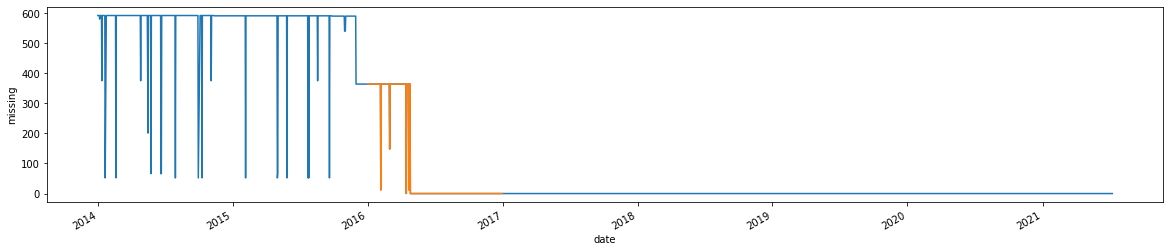
\includegraphics[width=6in]{images/missing_of_rain.png}
	\caption{Biểu đồ thể hiện dữ liệu bị thiếu, trục tung là số lượng xã bị mất dữ liệu lượng mưa}
\end{figure}

\subsubsection{Imputation of Data}

Bộ dữ liệu số 1 đầy đủ các thông tin cần thiết trong thời gian yêu cầu, nên việc imputation là không cần thiết.

Như đã nói thì phương pháp imputation ở đây là sử dụng dữ liệu lượng mưa ở thành phố trung tâm cho tất cả các xã bị mất dữ liệu. Ví dụ tất cả các xã của tỉnh Lâm Đồng bị mất dữ liệu lượng mưa/nhiệt độ trong ngày 20/8/2020 sẽ được lấp bằng dữ liệu lượng mưa/nhiệt độ của Đà Lạt ngày 20/8/2020.

Để thực hiện Imputation bộ dữ liệu thứ 2, ta map toàn bộ các tên các thành phố trong bộ dữ liệu WWO thành tên Tỉnh mà thành phố đó trực thuộc
\begin{minted}[breaklines, tabsize=4]{python}
df_wwo_weather_tn = df_wwo_weather[df_wwo_weather['province'].isin(['Buon Me Thuot','Play Cu','Da Lat'])].copy()
df_wwo_weather_tn['province'] = df_wwo_weather_tn['province'].replace({
    'Buon Me Thuot':'Đắk Lắk',
    'Play Cu':'Gia Lai',
    'Da Lat':'Lâm Đồng',
})
\end{minted}

Sau đó ta chuyển tên tỉnh đó thành mã tỉnh. Tạo một bảng chứa toàn bộ mã xã cùng với thời tiết của 3 tỉnh này từ bảng WWO. Merge bảng này với bảng dữ liệu từ weather.com bằng \texttt{left join} sau đó imputation từ cột của bảng WWO sang cột của bảng IBM weather ta sẽ được một bảng dữ liệu Imputation
\begin{minted}[breaklines,tabsize=2]{python}
# Create replacement df contain data imputation from wwo data to each ward of that province, drop province_code because don't need more
df_replacement = pd.merge(df_wwo_weather_tn, df_administrative_tn[['province_code', 'ward_code']], on=['province_code'], how='outer').dropna().drop(['province_code'], axis=1)

# Merge with ibm weather the for show missing data, drop ward because ward columns of IBM data will be NaN if ward do not have data in that date
df = pd.merge(df_ibm_weather, df_replacement, how='right', left_on=['ward','date'], right_on=['ward_code','date']).drop(['ward'], axis=1)

df['max_x'] = df['max_x'].fillna(df['max_y'])
df['min_x'] = df['min_x'].fillna(df['min_y'])
df['24_rain'] = df['24_rain'].fillna(df['rain'])
\end{minted}

\subsubsection{Creation of Dataset}

\qquad Việc tạo dữ liệu cho timeseries đã có hàm dựng sẵn từ tensorflow nên cách tạo dataset rất đơn giản, ta shuffle mã xã sau đó chia ra tùy vào mã xã. Lấy từng khoảng dữ liệu theo mã xã đã sắp xếp theo thời gian, đưa vào hàm \texttt{timeseries\_dataset\_from\_array}, sử dụng hàm \texttt{concatenate} ta sẽ tạo được các generator sử dụng cho việc training.

Tùy vào mục đích cho từng model ta sẽ cần mở rộng chiều của dữ liệu để phù hợp, ví dụ Conv2D sẽ yêu cầu dữ liệu 4 chiều. Việc sử dụng Generator sẽ kéo dài việc training song sẽ giúp quá trình tạo dataset vốn rất lớn gần như tức thời.
%----------------------------------------------------------------------------------------
%	SECTION 4
%----------------------------------------------------------------------------------------

\section{Training và đánh giá modelods}
% Chương này trình bày quá trình training và đánh giá các model mà nhóm đã thử. Đây là chương dài hơi và tốn thời gian nhất.
% Với mỗi model nhóm chọn thử nghiệm cần trình bày đầy đủ (1) nguồn tham khảo nếu như model đó tham khảo từ kết quả có trước. (2) Quá trình training thiết lập như thế nào, thời gian train, thời gian test, v.v..,

% Phần sau của chương trình bày kết quả đánh giá chi tiết model. Mỗi model phải show được các metric đánh giá performance.
% SHOW ĐƯỢC CÁC MẪU DỮ LIỆU mà model dự đoán sai và phân tích lý do. Đặc biệt chú ý các mẫu dữ liệu mà model này dự đoán đúng nhưng hầu hết model khác dự đoán sai, phải chụp ảnh được các mẫu dữ liệu đó làm ví dụ.
% Trình bày càng kỹ càng nhiều điểm

\subsection{Trên dữ liệu 5 tỉnh Tây Nguyên}
\subsubsection{Fully Connected}
\paragraph{Thiết lập, Training}
% Khúc này ghi cấu trúc model
% Thời gian training, thời gian test
% Nhớ ghi những thông số và công thức tính (acc, error, optimizor)

\paragraph{Đánh giá}
% Các đánh giá về model, số liệu tổng quan chung, các trường hợp model đoán đúng, sai,
% Còn những điểm nào có hy vọng cải thiện ?
% Bao quát chung

\subsubsection{Tổng kết}
% Rút ra gì từ những model khi thực nghiệm trên bộ dữ liệu này
% Trong các model này, những model nào có điểm tối ưu, hạn chế nào so với những model khác ?

\subsection{Trên dữ liệu 3 tỉnh (Gia Lai, Lâm Đồng, Đắk Lắk)}

Dữ liệu thời tiết được lấy từ năm 2014 đến 2020. Mỗi ngày lấy các thông tin thời tiết gồm các trường sau:

\begin{itemize}
	\item max\_temp: Nhiệt độ cao nhất trong ngày
	\item min\_temp: Nhiệt độ thấp nhất trong ngày
	\item wind\_x: Vector gió theo chiều x (được tạo thành từ hướng gió và tốc độ gió)
	\item wind\_y: Vector gió theo chiều y
	\item rain: Lượng mưa
	\item humidi: Độ ẩm
	\item Cloud: Tỷ lệ mây che phủ.
\end{itemize}

Với mỗi địa diểm xảy ra cháy trong một ngày nhất định thì ta lấy dữ liệu thời tiết (gồm các trường dữ liệu như trên) từ ngày trước khi xảy ra vụ cháy trở về trước 30 ngày. Với một ngày gồm 7 trường dữ liệu thời tiết trên ta nhân cho 30 ngày thì thu được 210 trường dữ liệu dùng để training.


\subsubsection{Model dữ đoán cháy rừng}
\paragraph{Chia dữ liệu}


Từ bộ dữ liệu đã được tạo ở trên, ta tiến hành chia dữ liệu thành các phần training, validation, testing. Ban đầu ta sẽ chia bộ dữ liệu thành training (70\%) và validation + testing (30\%). Sau đó từ bộ dữ liệu validation + testing, ta tiến hành chia dữ liệu thêm 1 lần nữa với tỷ lệ tương ứng là validation (70\%) và testing (30\%)

Sau khi chi dữ liệu xong ta có số lượng các bộ dữ liệu như sau:

\begin{itemize}
	\item Training dataset: 32921
	\item Validation dataset: 9876
	\item Testing dataset: 4233
\end{itemize}

\paragraph{Thiết lập, Training}
\subparagraph{Support Vector Machines (SVM)}


Ta sử dụng pipeline của thư viện sklearn để tiền xử lý dữ liệu và khởi tạo model SVM.

\begin{minted}[]{python}
	clf = make_pipeline(StandardScaler(), SVC(C=10, gamma='auto', kernel='rbf'))
\end{minted}

Trong SVC() ta thiết lập các thông số:
\begin{enumerate}
	\item C=1, gamma='auto', kernel='linear'
	      \begin{itemize}
		      \item Thời gian train: 9 min 28 second
		      \item Thời gian validation: 15 second
		      \item Thời gian test: 7 second
		      \item Accuracy:
		            \begin{itemize}
			            \item validation: 0.9590927501012556
			            \item testing: 0.9581856839121191
		            \end{itemize}
		      \item Mean Squared Error:
		            \begin{itemize}
			            \item validation: 0.04090724989874443
			            \item testing: 0.041814316087880936
		            \end{itemize}
	      \end{itemize}
	\item C=1, gamma='auto', kernel='rbf'
	      \begin{itemize}
		      \item Thời gian train: 41 second
		      \item Thời gian validation: 9 second
		      \item Thời gian test: 4 second
		      \item Accuracy:
		            \begin{itemize}
			            \item validation: 0.987444309437019
			            \item testing: 0.9877155681549729
		            \end{itemize}
		      \item Mean Squared Error:
		            \begin{itemize}
			            \item validation: 0.012555690562980963
			            \item testing: 0.012284431845027168
		            \end{itemize}
	      \end{itemize}
	\item C=10, gamma='auto', kernel='rbf'
	      \begin{itemize}
		      \item Thời gian train: 1 min 32 second
		      \item Thời gian validation: 8 second
		      \item Thời gian test: 4 second
		      \item Accuracy:
		            \begin{itemize}
			            \item validation: 0.9920008100445524
			            \item testing: 0.9943302622253721
		            \end{itemize}
		      \item Mean Squared Error:
		            \begin{itemize}
			            \item validation: 0.00799918995544755
			            \item testing: 0.005669737774627924
		            \end{itemize}
	      \end{itemize}
\end{enumerate}

Mean squared error được tính bằng công thức:
\begin{equation}
	MSE(y,\widehat{y}) = \frac{1}{n_samples} \sum_{i = 0}^{n_samples-1} (y_i - \widehat{y}_i)^2
\end{equation}
Trong đó:
\begin{itemize}
	\item $\widehat{y}$ là một tập các nhãn dự đoán
	\item $y$ là một tập các nhãn đúng
	\item $\widehat{y}$ là giá trị dữ đoán của mẫu thứ i
	\item $y_i$ là giá trị thực tương ứng với giá trị dự đoán trên
	\item $n_samples$ là số lượng các giá trị trong tập y (hoặc $\widehat{y}$)
\end{itemize}

\subparagraph{Dense}

Đầu tiên, ta khởi tạo model Sequential() của thự viện keras. Ta tiếp tục tạo lớp Input (đầu vào), và các lớp ẩn và cuối cùng là tạo lớp đầu ra. Trong lớp đầu vào ta cần khỏi tạo số nút tương ứng với kích thước của bộ dữ liệu. Trong các lớp ẩn thì ta cũng khởi tạo số nút cho mỗi lớp ẩn và thiết lập loại hình kích hoạt. Cuối cùng, trong lớp tạo số nút đầu ra và cũng thiết lập loại hình kích hoạt.

\begin{minted}[]{python}
	model = Sequential()
	model.add(Input(shape=(210,)))
	model.add(Dense(128, activation='relu', name='hidden_layer_1'))
	model.add(Dense(64, activation='relu', name='hidden_layer_2'))
	model.add(Dense(1, activation='sigmoid', name='output_layer'))
\end{minted}

Tiếp theo ta thiết lập hàm call back Early Stoping dùng để dừng quá trình train sớm, sau khi mà thông số chúng ta quan sát (có thể là validation accuarcy hay validation loss) không "khá lên" sau một vài epochs. Đây cũng là một kỹ thuật hay được dùng để tránh Overfit.

\begin{minted}[breaklines, tabsize=2]{python}
	callback = tf.keras.callbacks.EarlyStopping(monitor='val_loss', patience=5, mode='min')
\end{minted}

Tiếp tục ta tiếp hành lựa chọn các thuật toán tối ưu (optimizers). Về cơ bản, thuật toán tối ưu là cơ sở để xây dựng mô hình neural network với mục đích học được các features (hay pattern) của dữ liệu đầu vào, từ đó có thể tìm được một cặp weights và bias phù hợp để tối ưu hóa model. Trong các thuật toán tối ưu hóa ta tiến hành chọn learning rate (tỉ tệ học tập) sao cho phù hợp với bài toán.

\begin{minted}[]{python}
	sgd = SGD(learning_rate=0.01)
	
\end{minted}

Sau khi xây dựng model trên xong thì ta tiến hành comiple nó có tác dụng biên tập lại toàn bộ model của chúng ta đã xây dựng. Ở đây ta có thể lựa chọn các tham số để training model như: thuật toán training thông quan tham số optimize, hàm loss, chọn metrics hiện thị khi model được train.

\begin{minted}[]{python}
	model.compile(optimizer=sgd, loss='categorical_crossentropy',
              metrics=['accuracy'])
\end{minted}

Tiếp đến ta dùng hàm fit để đưa data vào training để tìm tham số model.

\begin{minted}[]{python}
	history = model.fit(X_train, y_train, batch_size=64, epochs=200, validation_data=(X_valid, y_valid), callbacks=callback, verbose=1).history
\end{minted}

Từ model đã được xây dựng trên, ta tiến hành chỉnh sửa các thông số của model:
\begin{enumerate}
	\item Hai lớp ẩn (số nút tương ứng là 128 và 64, activation="relu"), SGD(learning\_rate=0.01), loss="binary\_crossentropy"

	      \begin{itemize}
		      \item Thời gian train: 5 min 13 second
		      \item Thời gian validation: 27 second
		      \item Thời gian test: 5 second
		      \item Accuracy:
		            \begin{itemize}
			            \item validation: 0.9533211588859558
			            \item testing: 0.9588943719863892
		            \end{itemize}
		      \item Loss:
		            \begin{itemize}
			            \item validation: 0.15693733096122742
			            \item testing: 0.1464112251996994
		            \end{itemize}
		      \item Mean Squared Error:
		            \begin{itemize}
			            \item validation: 0.042361213827923364
			            \item testing: 0.03825463792437562
		            \end{itemize}
	      \end{itemize}
	\item Hai lớp ẩn (số nút tương ứng là 128 và 64, activation="relu"), optimizer="adam", loss="binary\_crossentropy"
	      \begin{itemize}
		      \item Thời gian train: 5 min 13 second
		      \item Thời gian validation: 7 second
		      \item Thời gian test: 5 second
		      \item Accuracy:
		            \begin{itemize}
			            \item validation: 0.9870392680168152
			            \item testing: 0.9893692135810852
		            \end{itemize}
		      \item Loss:
		            \begin{itemize}
			            \item validation: 0.059234291315078735
			            \item testing: 0.046542562544345856
		            \end{itemize}
		      \item Mean Squared Error:
		            \begin{itemize}
			            \item validation: 0.011526199238160804
			            \item testing: 0.009204111539974925
		            \end{itemize}
	      \end{itemize}
	\item Ba lớp ẩn (số nút tương ứng là 128, 64 và 32, activation="relu"), optimizer="adam", loss="binary\_crossentropy"
	      \begin{itemize}
		      \item Thời gian train: 3 min 23 second
		      \item Thời gian validation: 2 second
		      \item Thời gian test: 1 second
		      \item Accuracy:
		            \begin{itemize}
			            \item validation: 0.990481972694397
			            \item testing: 0.9922041296958923
		            \end{itemize}
		      \item Loss:
		            \begin{itemize}
			            \item validation: 0.0414808988571167
			            \item testing: 0.037396930158138275
		            \end{itemize}
		      \item Mean Squared Error:
		            \begin{itemize}
			            \item validation: 0.00846018838163131
			            \item testing: 0.00734131887253742
		            \end{itemize}
	      \end{itemize}
\end{enumerate}

\begin{figure}[H]
	\centering
	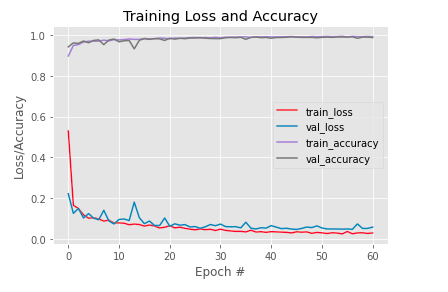
\includegraphics[width=6in]{images/loss_acc_model1_0.png}
	\caption{Biểu đồ thể hiện quá trình training}
\end{figure}

\paragraph{Đánh giá}

Từ hai thuật toán phân loại phân loại trên ta thấy được model hình dự đoán khá tốt khi dự báo cháy rừng trên dữ liệu thời tiết. Cụ thể , đốí với model SVM cho ra accuracy đối với tập dữ liệu validation là 99,2\% và dữ liệu testing thì 99,43\%. Còn model Dense thì cho ra accuracy đối với tập dữ liệu validation là 99,05\% và dữ liệu testing thì 99,22\%


%\paragraph{Tổng kết}

\subsubsection{Model dự đoán cấp độ cháy rừng}

Model này dùng để dự đoán các cấp độ cháy rừng sau khi đã có kết quả của model trên. Nếu model dự báo cháy rừng trên cho ra kết quả là 1 (tương ứng với việc có xảy ra cháy rừng) thì ta tiếp tục sử dụng model này để  phân loại các cấp độ cháy rừng, để có thể kịp thời ứng phó với nguy cơ cháy rừng. Còn nếu model trên dự đoán ra 0 thì ta không cần phải dự đoán tiếp model này.

\paragraph{Chia dữ liệu}

Tương tự như model trên viêc chia dữ liệu cũng giống tưng tự. Sau khi chi dữ liệu xong ta có số lượng các bộ dữ liệu như sau:

\begin{itemize}
	\item Training dataset: 17311
	\item Validation dataset: 5193
	\item Testing dataset: 2226
\end{itemize}

\paragraph{Thiết lập, Training}

\subparagraph{Support Vector Machines (SVM)}

Tương tự như SVM của model trên ta cũng tiến hành thiết lập model và thay đổi các thông số để cho ra kết quả mong muốn:

\begin{enumerate}
	\item C=1, gamma='auto', kernel='poly'
	      \begin{itemize}
		      \item Thời gian train: 2 min 8 second
		      \item Thời gian validation: 25 second
		      \item Thời gian test: 12 second
		      \item Accuracy:
		            \begin{itemize}
			            \item validation: 0.6187175043327556
			            \item testing: 0.6154537286612758
		            \end{itemize}
		      \item Mean Squared Error:
		            \begin{itemize}
			            \item validation: 0.7232813402657423
			            \item testing: 0.7497753818508536
		            \end{itemize}
	      \end{itemize}
	\item C=1, gamma='auto', kernel='rbf'
	      \begin{itemize}
		      \item Thời gian train: 1 min 56 second
		      \item Thời gian validation: 27 second
		      \item Thời gian test: 11 second
		      \item Accuracy:
		            \begin{itemize}
			            \item validation: 0.6347005584440593
			            \item testing: 0.6302785265049416
		            \end{itemize}
		      \item Mean Squared Error:
		            \begin{itemize}
			            \item validation: 0.6761024455998459
			            \item testing: 0.7133872416891285
		            \end{itemize}
		            \begin{figure}[H]
			            \centering
			            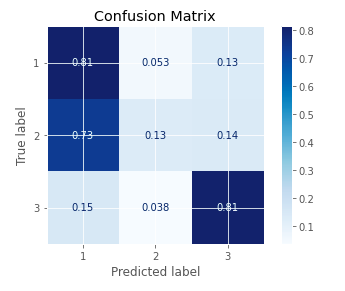
\includegraphics[width=6in]{images/confusionMatrixSVM_model2_0.png}
			            \caption{Confusion Matrix}
		            \end{figure}
	      \end{itemize}
\end{enumerate}

\subparagraph{Dense}

Ta thiết lập model tương tự model trên:

\begin{minted}[breaklines,tabsize=4]{python}
	model = Sequential()
	model.add(Dense(128, input_shape=(210,), activation="relu", name='hidden_layer_1'))
	model.add(Dense(64, activation="relu", name='hidden_layer_2'))
	model.add(Dense(32, activation="relu", name='hidden_layer_3'))
	model.add(Dense(16, activation="relu", name='hidden_layer_4'))
	model.add(Dense(3, activation="sigmoid", name='output_layer'))

	callback = tf.keras.callbacks.EarlyStopping(monitor='val_loss', patience=10, mode='min')

	model.compile(optimizer='adam', loss='categorical_crossentropy',
              metrics=['accuracy'])
	
	history = model.fit(X_train, y_train, batch_size=64, epochs=200, validation_data=(X_valid, y_valid), callbacks=callback, verbose=1)
\end{minted}

\begin{itemize}
	\item Thời gian train: 1 min 4 second
	\item Thời gian validation: 5 second
	\item Thời gian test: 2 second
	\item Accuracy:
	      \begin{itemize}
		      \item validation: 0.6192951798439026
		      \item testing: 0.6145552396774292]
	      \end{itemize}
	\item Loss:
	      \begin{itemize}
		      \item validation: 0.8435102105140686
		      \item testing: 0.8677495121955872
	      \end{itemize}
	\item Mean Squared Error:
	      \begin{itemize}
		      \item validation: 0.16747459320485225
		      \item testing: 0.17110031298128617
	      \end{itemize}
\end{itemize}

\begin{figure}[H]
	\centering
	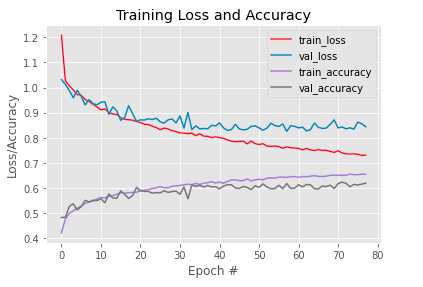
\includegraphics[width=6in]{images/loss_acc_model2_0.png}
	\caption{Biểu đồ thể hiện quá trình training}
\end{figure}

Từ model trên, ta thấy được nhãn 2 dự đoán đúng rất thấp, chủ yếu lệch về phía nhãn 1 rất nhiều, vì vật để khắc phục vấn đề này ta tiến hành giảm lớp class xuống, chỉ còn 2 lớp (nhãn 1, 2) và tiến hành phân chia lại dữ liệu. Thực ra, ban đầu nhóm chia dữ liệu cháy thành 3 lớp là dự trên số lượng các điểm cháy xảy ra trong ngày ở một xã nhất định. Vì theo quan điểm của nhóm thì số lượng điểm cháy xảy ở một xã trong một ngày càng nhiều thì cho thấy dữ liệu thời tiết đó càng có nguy cơ cao xảy ra cháy rừng. Nhưng sau khi phân chia dữ liệu, tiến hành train thì xảy ra hiện tượng trên, dữ liệu không khớp khi với nhãn 2, phần lớn những dữ liệu đó thì dễ nhầm với nhãn 1 hơn nên nhóm mới quyết định gộp nhãn 1 với nhãn 2 cũ thành nhãn 1 mới và chuyển nhãn 3 thành nhãn 2. Ta tiến hành train với dữ liệu mới. Sau khi train với nhiều model khác nhau, ta có kết quả các model như sau:

\subparagraph{Support Vector Machines (SVM)}

Trong SVC() ta thiết lập các thông số:
\begin{enumerate}
	\item C=1, gamma='auto', kernel='rbf'
	      \begin{itemize}
		      \item Thời gian train: 1 mini 29 second
		      \item Thời gian validation: 19 second
		      \item Thời gian test: 8 second
		      \item Accuracy:
		            \begin{itemize}
			            \item validation: 0.8239938378586559
			            \item testing: 0.8221024258760108
		            \end{itemize}
		      \item Mean Squared Error:
		            \begin{itemize}
			            \item validation: 0.17600616214134412
			            \item testing: 0.1778975741239892
		            \end{itemize}
	      \end{itemize}
	\item C=10, gamma='auto', kernel='rbf'
	      \begin{itemize}
		      \item Thời gian train: 2 min 20 second
		      \item Thời gian validation: 17 second
		      \item Thời gian test: 7 second
		      \item Accuracy:
		            \begin{itemize}
			            \item validation: 0.8234161371076449
			            \item testing: 0.8274932614555256
		            \end{itemize}
		      \item Mean Squared Error:
		            \begin{itemize}
			            \item validation: 0.1765838628923551
			            \item testing: 0.1725067385444744
		            \end{itemize}
	      \end{itemize}
\end{enumerate}

\begin{figure}[H]
	\centering
	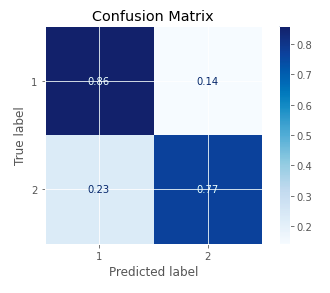
\includegraphics[width=6in]{images/confusionMatrixSVM_model2_1.png}
	\caption{Confusion Matrix}
\end{figure}

\subparagraph{Dense}

Tương tự, ta chỉ xét đến các thông số sau khi train xong model:

\begin{itemize}
	\item Thời gian train: 2 min 6 second
	\item Thời gian validation: 5 second
	\item Thời gian test: 2 second
	\item Accuracy:
	      \begin{itemize}
		      \item validation: 0.8137878179550171
		      \item testing: 0.8126684427261353
	      \end{itemize}
	\item Loss:
	      \begin{itemize}
		      \item validation: 0.4617549777030945
		      \item testing: 0.46853387355804443
	      \end{itemize}
	\item Mean Squared Error:
	      \begin{itemize}
		      \item validation: 0.14147366984777401
		      \item testing: 0.14031667554728067
	      \end{itemize}
\end{itemize}

\begin{figure}[H]
	\centering
	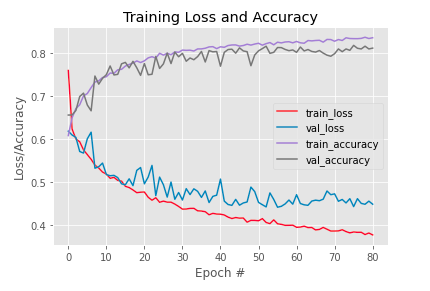
\includegraphics[width=6in]{images/loss_acc_model2_1.png}
	\caption{Biểu đồ thể hiện quá trình training}
\end{figure}

\paragraph{Đánh giá}

Nhìn chung model được chia thành 3 lớp dựa trên số điểm cháy của xã trong một ngày ban đầu cho ra kết quả khá tệ, nó chỉ dự đoán tốt trên nhãn 1 và nhãn 3 (81\% và 81\%) còn nhãn 2 thì cho ra kết quả khá tệ(13\%), các dự đoán gần như là rơi vào nhẵn 1 (chiếm đến 73\%).

Khi xây dựng lại bộ dữ liệu 2 lớp thì cho ra kết quả khả quan hơn với accuracy là 82,39\% đối với dữ liệu validation và 82,21\% đối với dữ liệu testing. Mặc dù khi giảm số class thì accuracy sẽ tăng lên, dẫn đến phân loại đúng hơn. Nhưng cũng phải chấp nhận phương pháp trên, việc phân chia số lượng class trên còn phải dựa vào số lượng dữ liệu điểm cháy nữa nên không thể tạo thành nhiều lớp hơn khi gộp dữ liệu nhãn 1 và 2 trên lại với nhau. Vì vậy, nhóm quyết định chỉ làm 2 lớp để phân loại.

%\paragraph{Tổng kết}
\subsubsection{Tổng kết}

Qua quá trình đào tạo 2 mô hình khác nhau, với độ dữ đoán chính xác là khác nhau. Mô hình đầu tiên cho kết quả tốt trên cả tập train, tập validation và tập test. Loss thấp và mean squared error cũng khá thấp, cho thấp khả năng học tập và đào tạo của mô hình là khá tốt. Từ đó thấy được mô hình dữ đoán cháy rừng có thể áp dụng thực tế được. Mặc dù, nhóm chưa thử kiểm tra với dữ liệu năm 2021 (vì dữ liệu thời tiết thì có thể thu thập, nhưng dữ liệu cháy rừng năm 2021 thì chưa có nên khi dữ đoán thì không thể kiểm tra đươc nên nhóm chưa trên khai kiểm tra thử) nhưng với độ chính xác cao thì nó vẫn có khả năng lớn là cho ra kết quả dữ đoán đúng về việc xảy ra cháy rừng trên địa bàn tỉnh Tây Nguyên.

Mô hình thử hai dự đoán cấp độ cháy rừng cho kết quả thấp với việc phân chia dữ liệu thành 3 lớp, nhưng khi thấy vấn đề ở việc phân chia dữ như vậy, thì nhóm quyết định giảm lớp phân loại xuống còn hai lớp và tiến hành phân chia lại dữ liệu thì cho ra kết qủa khả quan hơn với độ chính xác trên 80\%, điều này làm cho việc kiểm tra phân loại cấp độ cháy cho độ chính xác cao hơn và có thể thử nghiệm thử trong thực tế.

%----------------------------------------------------------------------------------------
%	SECTION 5

% Chương cuối trình bày khả năng ứng dụng của model, và hướng phát triển tiếp theo. Sẽ có điểm cộng nếu nhóm xây dựng được ứng dụng minh họa thực tế từ model đã train.

%----------------------------------------------------------------------------------------

\section{Ứng dụng và hướng phát triển}

\begin{itemize}
	\item Sử dụng Deep learning để imputation dữ liệu còn thiếu
	\item Tìm thêm nhiều nguồn dữ liệu thời tiết
	\item Nghiên cứu sử dụng multiple input
\end{itemize}


%----------------------------------------------------------------------------------------
%	BIBLIOGRAPHY
%----------------------------------------------------------------------------------------

\bibliographystyle{plain}
\bibliography{source}

%----------------------------------------------------------------------------------------

\end{document}